\documentclass[a4paper, 12pt]{article}
\usepackage[a4paper,top=1.5cm, bottom=1.5cm, left=1cm, right=1cm]{geometry}
\usepackage[utf8]{inputenc}
\usepackage{mathtext}
\usepackage{amsmath}
\usepackage{amsfonts}
\usepackage[english, russian]{babel}
\usepackage{indentfirst}
\usepackage{longtable}
\usepackage{graphicx}
\usepackage{tabularx}
\graphicspath{{images/}}
\DeclareGraphicsExtensions{.pdf,.png,.jpg}
\usepackage{natbib}


\usepackage{float}  % принудительное размещение таблицы ко кодовой букве H вместо !ht
\restylefloat{table}

\usepackage{letltxmacro}  % новый дизайн корня(с закорючкой вниз на конце)
\makeatletter
\let\oldr@@t\r@@t
\def\r@@t#1#2{
\setbox0=\hbox{$\oldr@@t#1{#2\,}$}\dimen0=\ht0
\advance\dimen0-0.2\ht0
\setbox2=\hbox{\vrule height\ht0 depth -\dimen0}
{\box0\lower0.4pt\box2}}
\LetLtxMacro{\oldsqrt}{\sqrt}
\renewcommand*{\sqrt}[2][\ ]{\oldsqrt[#1]{#2} }
\makeatother

\usepackage{wrapfig}  % рисунки с обтеканием

\usepackage{color,soul}  % новая команда \ul - подчеркивание красной линией
\setulcolor{red} 

\usepackage{breqn} % пак для создания двустрочных equation через \begin{dmath}

\usepackage{nicematrix}  % цветные таблиц


\title{Лабораторная работа \\ Газоразрядный стабиловольт.}
\author{Волков Роман, Виноградов Кирилл, Зайцев Дмитрий}
\date{29 марта 2024 г.}


\begin{document}

%\numberwithin{equation}{section}

% \renewcommand{\cftsecleader}{\cftdotfill{\cftdotsep}} % добавляем точки между номером раздела и его названием

\setcounter{page}{2} % Начало отсчета страниц с 2
\tableofcontents  % Оглавление
	\newpage
	
\section*{\textbf{Цель работы:}}
\addcontentsline{toc}{section}{Цель работы}

1) Изучить принципы работы газоразрядного стабилизатора напряжения
(стабиловольта);\par
2) Получить кривые Пашена при разных рабочих газах;\par
3) Получить вольт-амперную характеристику стабиловольта;\\


\section*{\textbf{Схема установки}}
\addcontentsline{toc}{section}{Схема установки}
	
	

    \begin{figure}[H]
        \centering
        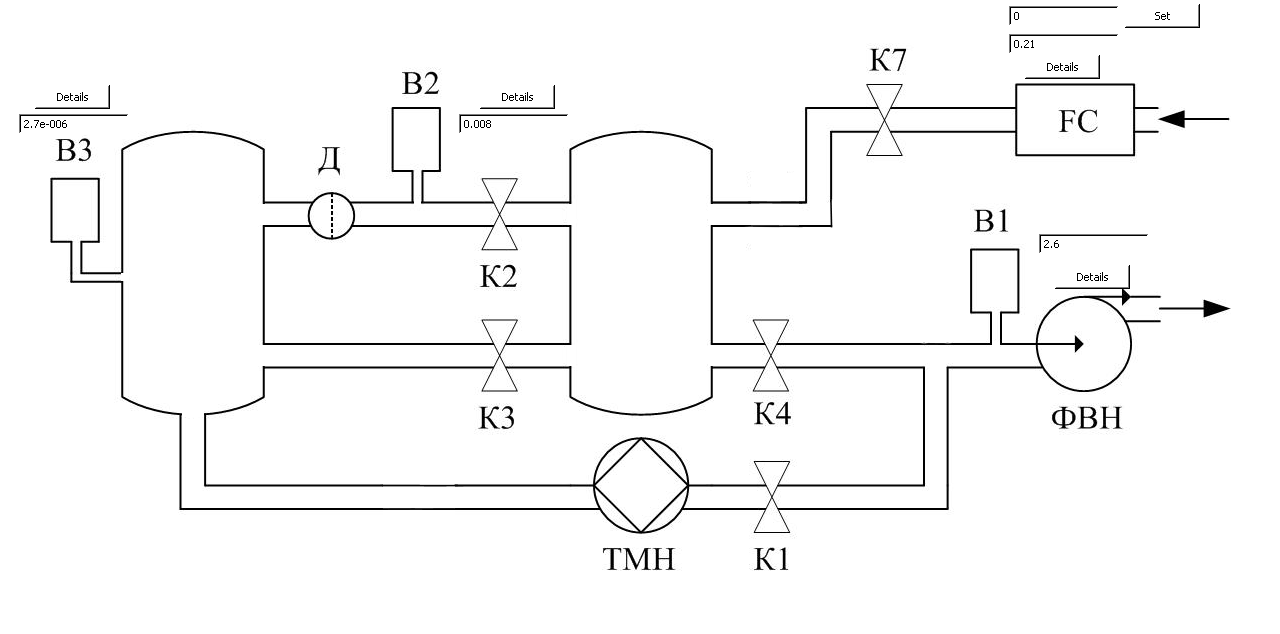
\includegraphics[width=1\linewidth]{scheme.png}
        \caption{Схема лабораторной установки: В1 – вакууметр ёмкостной; В2 – вакууметр терморезистивный; В3 – вакууметр ионизационный; К1 – кран турбомолекулярного насоса; К2 – комутационный кран; К3 – высоковакуумная заслонка; К4 – форвакуумная заслонка; Д –диафрагма; FC – регулятор газового потока; ТМН – турбомолекулярный насос; ФВН – форвакуумный насос}
        \label{img_device}
    \end{figure}

 В работе откачка системы производится механическим вращательным
пластинчато-роторным насосом ФВН, соединённым с системой
гофрированным шлангом. Давление в рабочей камере измеряется при
помощи терморезистивного вакууметра В2.

\section*{ВАХ газоразрядного диода}
\addcontentsline{toc}{section}{ВАХ газоразрядного диода}
	
Протекание тока через газовый разряд представляет собой комплексное
явление, протекающее по разным механизмам и зависящее от множества
внешних параметров. Поэтому ВАХ газоразрядного диода представляет
собой довольно сложную зависимость, представленную на рисунке 2.
Участок 1 характеристики соответствует несамостоятельному разряду; 2 –
несамостоятельному разряду, но с газовым усилением; 3 – соответствует
переходу к тлеющему разряду; 4 – нормальному тлеющему разряду; 5 –
аномальному тлеющему разряду; 6 – переходу разряда в дуговой; 7 –
дуговому разряду, для которого характерна термоэмиссия электронов из
раскалённого катода.

	
    \begin{figure}[H]
        \centering
        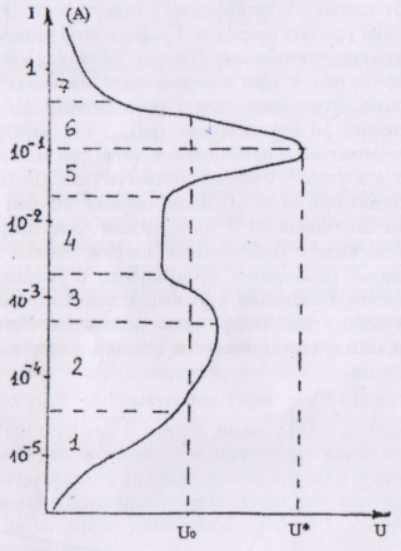
\includegraphics[width=0.5\linewidth]{vax.png}
        \caption{ВАХ газоразрядного диода.}
        \label{img_}
    \end{figure}


\section*{\textbf{Ход работы}}
\addcontentsline{toc}{section}{Ход работы}
	
1) Включаем компьютер и подаём питание на установку.

2) Приводим установку в рабочее состояние. Все краны открыты. В
установке атмосферное давление. Колбу на установке подсоединяем к
источнику напряжения (на схеме не показан).

3) Включаем источник напряжения, терморезистивный вакууметр В2,
регулятор газового потока FC и устанавливаем начальный поток газа
равным 100 sccm.

4) Включаем форвакуумный насос, ожидаем пока в системе не
установится постоянное давление.

5) Снимаем зависимость напряжения газоразрядного промежутка от
давления в колбе. Результаты занесём в таблицу 1..


\begin{table}[h!]
\centering
\caption{Данные, отсортированные по s от 100 до 8}
% resizebox растягивает таблицу на всю ширину текста (\textwidth)
\resizebox{\textwidth}{!}{%
\begin{tabular}{|c|c|c|c|c|c|c|c|c|c|c|c|c|c|c|c|c|c|c|c|c|c|}
\hline
$P, \text{торр}$ & 0,223 & 0,206 & 0,190 & 0,172 & 0,155 & 0,136 & 0,500 & 1,200 & 1,850 & 2,540 & 2,830 & 0,116 & 0,095 & 0,084 & 0,072 & 0,058 & 0,051 & 0,042 & 0,038 & 0,035 & 0,034 \\ \hline
$U, 10^{-2} \text{кВ}$ & 60 & 59 & 59 & 60 & 60 & 67 & 60 & 70 & 80 & 90 & 94 & 73 & 85 & 96 & 109 & 130 & 142 & 160 & 205 & 260 & 263 \\ \hline
\end{tabular}%
}
\end{table}

6) По полученным данным строим график соответствующей зависимости.
Погрешности приборов принимаются равными половине последнего
разряда. P0 - давление, соответствующее минимальному напряжению.
	
7) Установим в камере давление, соответствующее минимальному
значению напряжения (0.17 торр), и снимем ВАХ стабиловольта.
Результаты занесём в таблицу 2 и построим график соотетствующей
зависимости (рисунок 4).



    \begin{figure}[H]
        \centering
        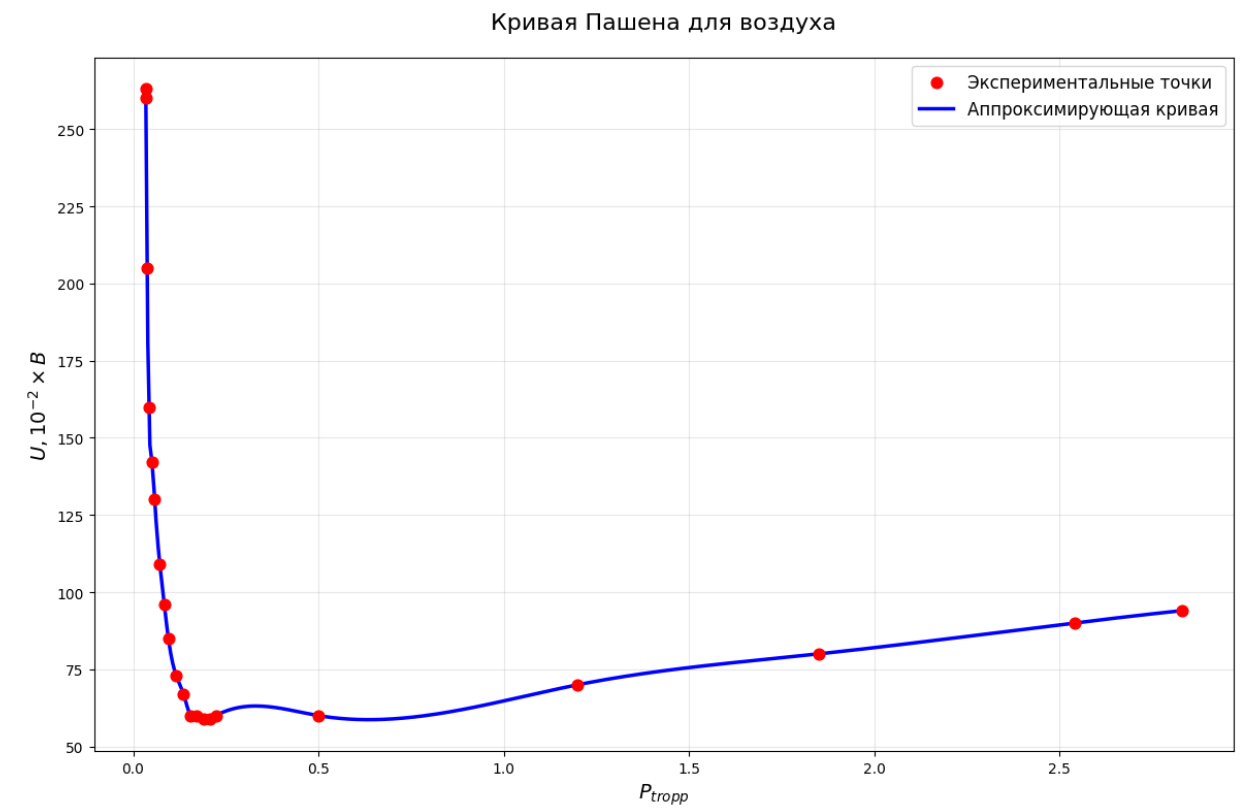
\includegraphics[width=0.7\linewidth]{1.png}
        \caption{График зависимости напряжения газоразрядного промежутка от давления
    воздуха в колбе (кривая Пашена).}
        \label{img_1}
    \end{figure}

 

Вольт-амперная характеристика стабиловольта для воздуха:\par
\begin{tabular}{|c|c|c|c|c|c|c|c|c|c|c|}
\hline
$I$, $10^{-4}$ А & 19 & 17 & 15 & 13 & 11 & 9 & 7 & 5 & 3 & 1 \\
\hline
$U$, $10^{-2}$ кВ & 59 & 59 & 60 & 61 & 62 & 62 & 63 & 65 & 69 & 67 \\
\hline
\end{tabular}

    \begin{figure}[H]
        \centering
        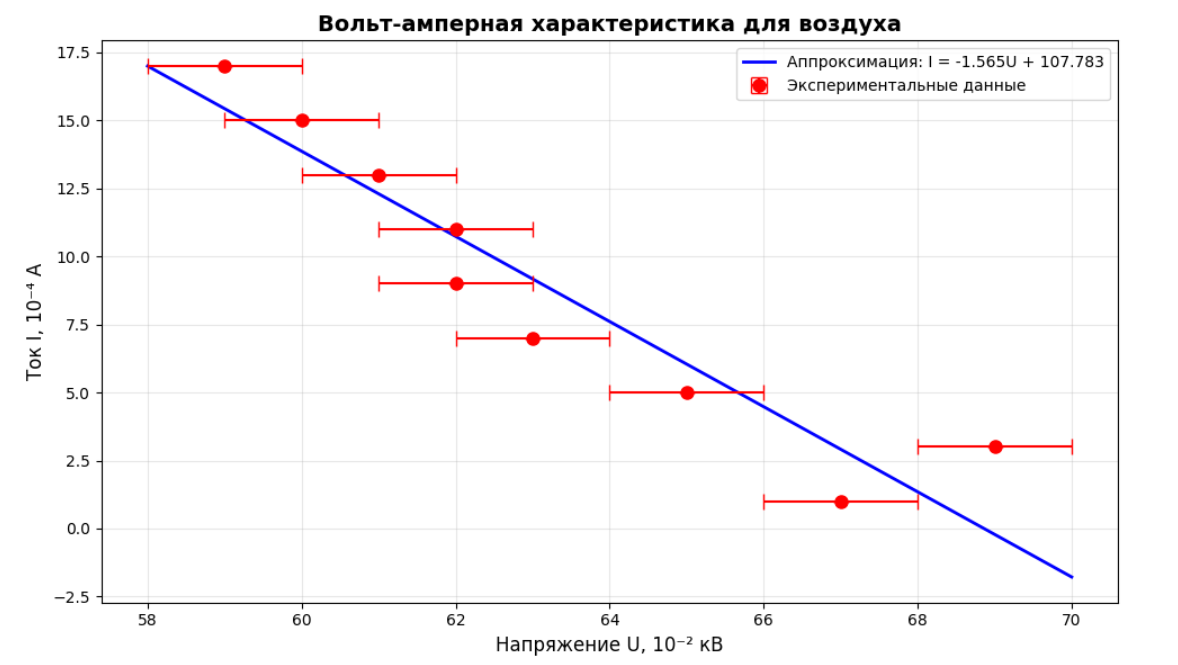
\includegraphics[width=1\linewidth]{4.png}
        \caption{Вольт-амперная характеристика стабиловольта для воздуха.}
        \label{img_4}
    \end{figure}

8) Заместим воздух в системе аргоном и повторим действия п. 5) - 7).



\begin{table}[h]
\centering
\scriptsize
\setlength{\tabcolsep}{2pt}
\begin{tabular}{|l|*{18}{c|}}
\hline
$P$, торр & 0,7 & 2,15 & 2,5 & 0,192 & 0,178 & 0,163 & 0,117 & 0,082 & 0,071 & 0,067 & 0,063 & 0,061 & 0,062 & 0,057 & 0,051 & 0,05 & 0,045 & 0,033 \\
\hline
$U$, $10^{-2}$ кВ & 45 & 50 & 55 & 41 & 41 & 41 & 41 & 41 & 41 & 73 & 79 & 81 & 80 & 88 & 96 & 100 & 113 & 154 \\
\hline
\end{tabular}
\caption{Зависимость напряжения газоразрядного промежутка от давления в колбе для аргона.}
\label{tab:p_u}
\end{table}




\begin{table}[h]
\centering
\begin{tabular}{|c|c|c|c|c|c|c|c|c|c|c|c|c|c|c|c|c|c|c|c|}
\hline
$I,\ 10^{-4}\ \text{A}$ & 19 & 18 & 17 & 16 & 15 & 14 & 13 & 12 & 11 & 10 & 9 & 8 & 7 & 6 & 5 & 4 & 3 & 2 & 1 \\
\hline
$U,\ 10^{-2}\ \text{кВ}$ & 41 & 41 & 41 & 41 & 41 & 42 & 42 & 47 & 48 & 48 & 48 & 49 & 50 & 50 & 51 & 51 & 52 & 52 & 52 \\
\hline
\end{tabular}
\caption{Вольт-амперная характеристика стабиловольта для аргона.    }
\label{tab:IU}
\end{table}
    

    \begin{figure}[H]
        \centering
        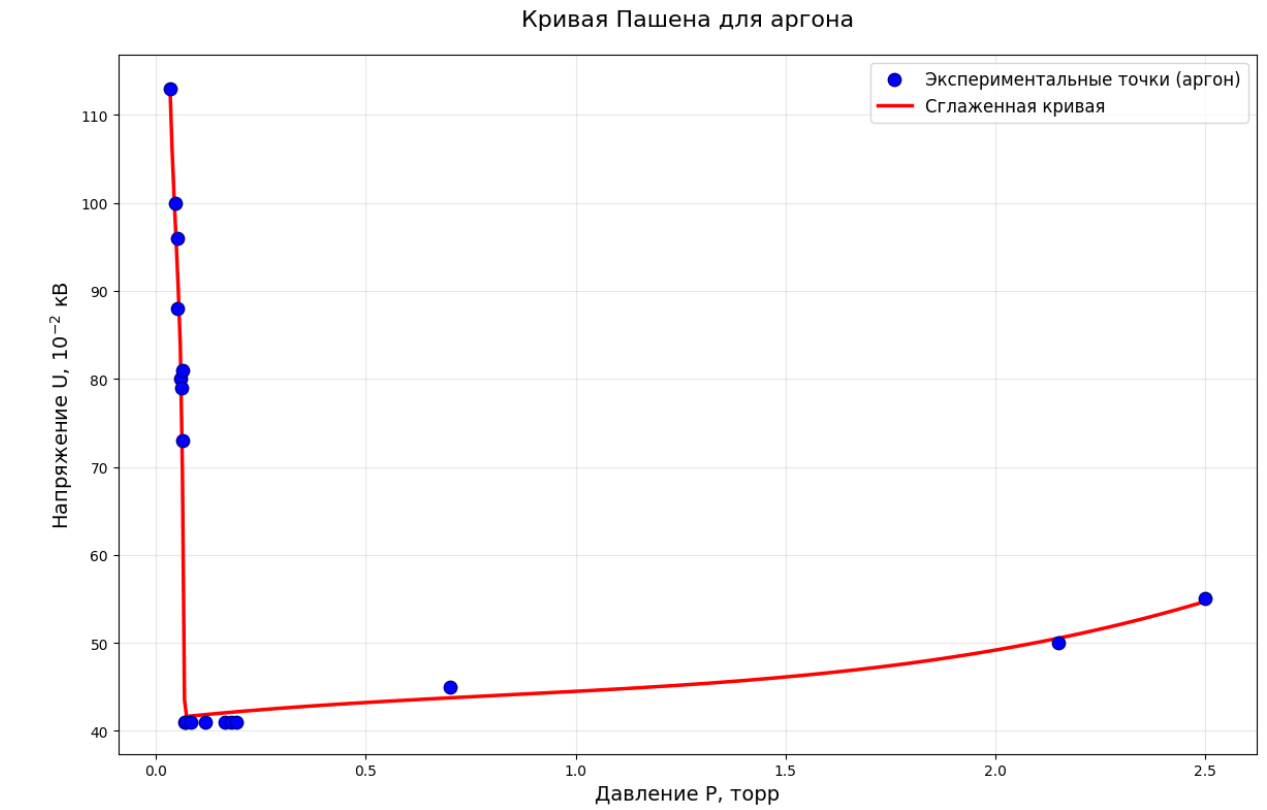
\includegraphics[width=0.8\linewidth]{2.png}
        \caption{График зависимости напряжения газоразрядного промежутка от давления
    аргона в колбе (кривая Пашена).}
        \label{img_2}
    \end{figure}

    \begin{figure}[H]
        \centering
        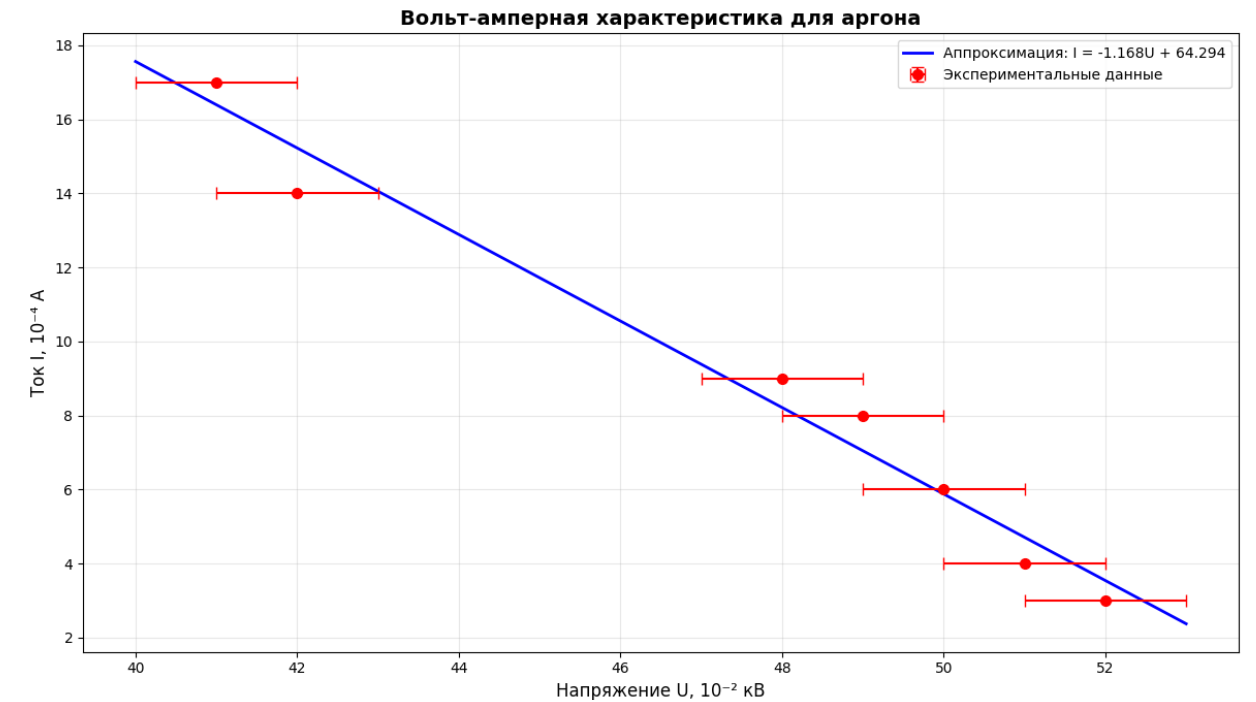
\includegraphics[width=0.8\linewidth]{5.png}
        \caption{Вольт-амперная характеристика стабиловольта для аргона.}
        \label{img_5}
    \end{figure}

 	
9) Поместим кривые Пашена и ВАХ воздуха и аргона на одни графики. Видно, что кривые Пашена, полученные экспериментально имеют вид типичных кривых Пашена, что говорит о применимости теории в нашем случае.
    
    \begin{figure}[H]
        \centering
        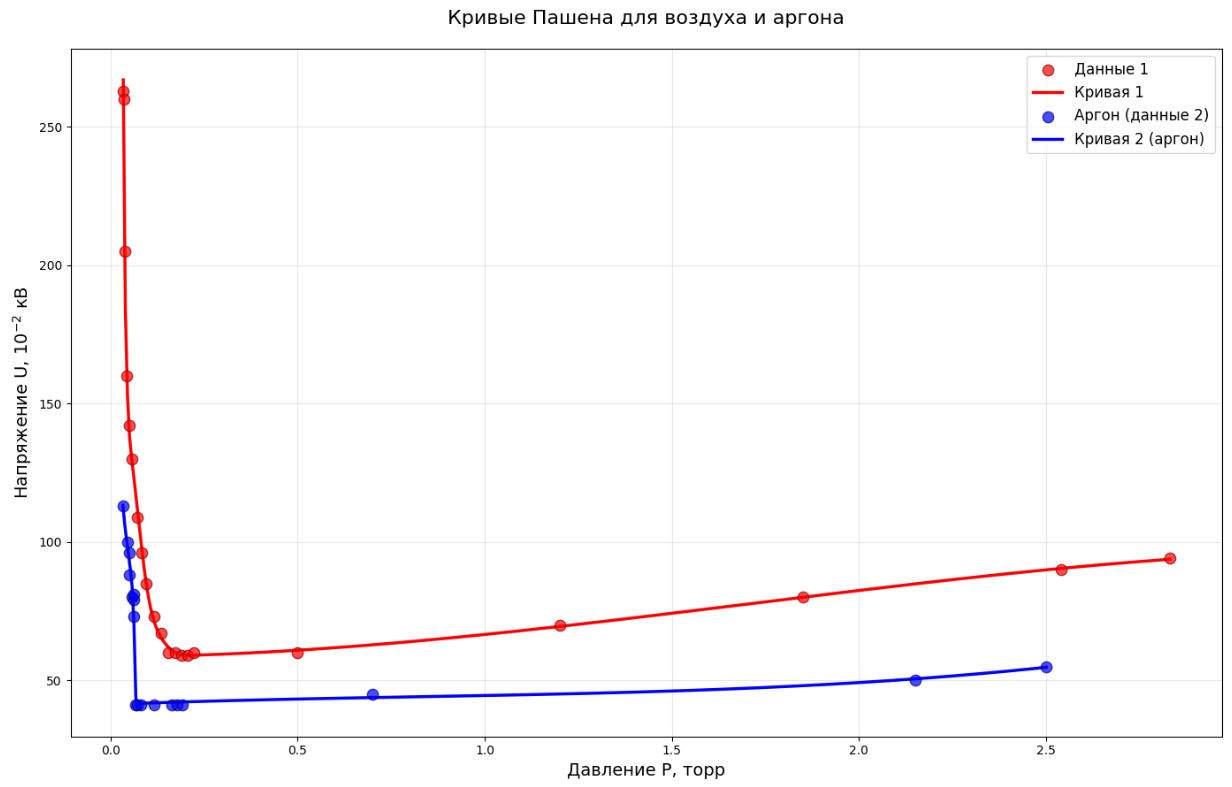
\includegraphics[width=0.8\linewidth]{3.png}
        \caption{Кривые Пашена для воздуха и аргона.}
        \label{img_3}
    \end{figure}

    \begin{figure}[H]
        \centering
        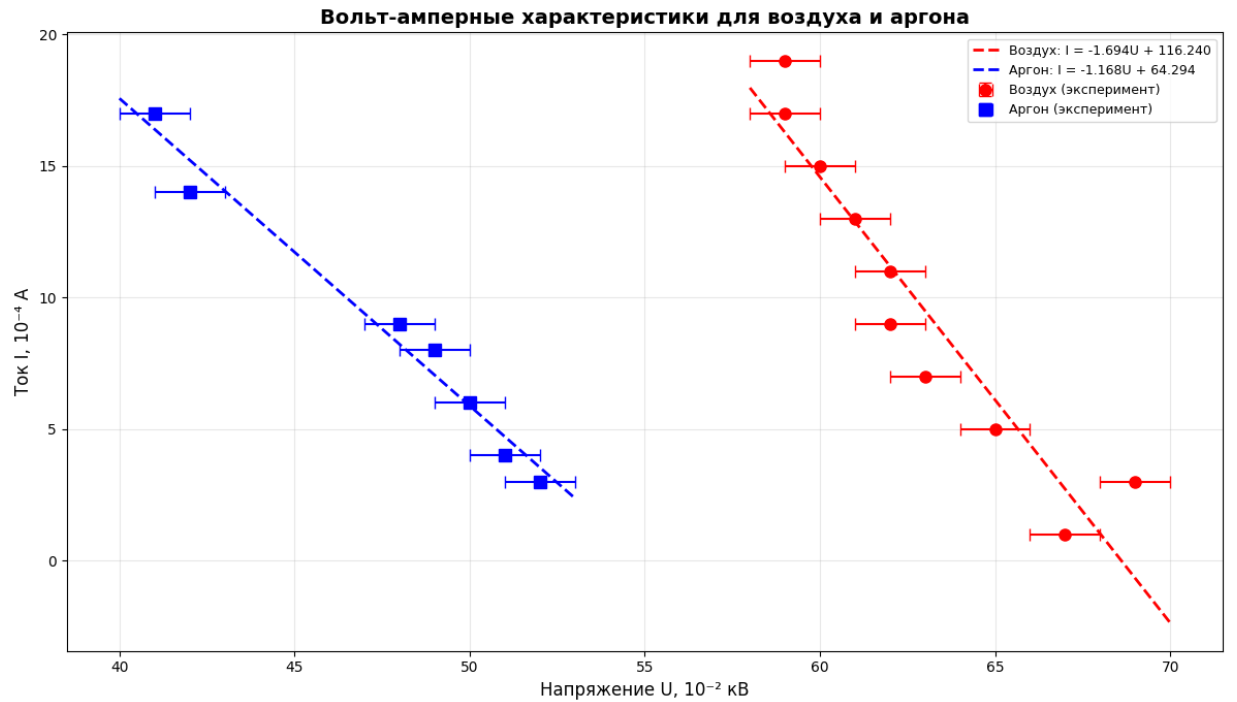
\includegraphics[width=0.8\linewidth]{6.png}
        \caption{Вольт-амперные характеристики стабиловольта для воздуха и аргона.}
        \label{img_6}
    \end{figure}

    
10) По значениям тока и напряжения, а также по общему виду ВАХ
можно утверждать, что они соответствуют участку 3 на рисунке 2, то
есть переходу к тлеющему разряду. Вычисление коэффициента
стабилизации по полученным данным невозможно, поскольку
стабиловольт не вышел на рабочий режим (участок 4 на рисунке 2).

\section*{\textbf{Заключение}}
\addcontentsline{toc}{section}{Заключение}

В результате выполнения работы:

1) Изучены принципы работы газоразрядного стабилизатора напряжения.

2) Получены кривые Пашена при заполнении колбы воздухом и аргоном. Полученные кривые имеют вид, типичный для данной зависимости.

3) Получены вольт-амперные характеристики стабиловольта при заполнении его воздухом и аргоном. По кривым установлено, что режим газового разряда, полученный в работе - переход к тлеющему разряду.

\end{document}

    \begin{figure}[H]
        \centering
        \includegraphics[width=1\linewidth]{images/ .png}
        \caption{.}
        \label{img_}
    \end{figure}